\documentclass[a4paper,twoside]{report}
\usepackage[landscape,margin=1in]{geometry}
\usepackage{color}
\usepackage[final]{flowfram}
\usepackage[colorlinks]{hyperref}
\usepackage{graphicx}
\usepackage{helvet}
\usepackage{calc}
\usepackage{chemfig}
\usepackage[version=3]{mhchem}
\usepackage{booktabs}
\usepackage{colortbl}
\usepackage[export]{adjustbox}[2011/08/13]
\usepackage{datatool}

\usepackage{lipsum}

%%%%%%%%%%%%%%%%%%%%%%%
%  TRIUMF COLOURS
%%%%%%%%%%%%%%%%%%%%%%%
% primary
\definecolor{TRIUMFcyan}{RGB}{0,159,223}
\definecolor{TRIUMFwhite}{RGB}{255,255,255}
\definecolor{TRIUMFblack}{RGB}{17,17,17}

% secondary
\definecolor{TRIUMFdarkgray}{RGB}{128,130,133}
\definecolor{TRIUMFmediumgray}{RGB}{209,211,212} 
\definecolor{TRIUMFlightgray}{RGB}{241,242,242}
\definecolor{TRIUMFyellow}{RGB}{225,203,5}
%duplicate to avoid errors on gray/grey spelling...
\definecolor{TRIUMFdarkgrey}{RGB}{128,130,133}
\definecolor{TRIUMFmediumgrey}{RGB}{209,211,212} 
\definecolor{TRIUMFlightgrey}{RGB}{241,242,242}

% tertiary
\definecolor{TRIUMFgreen}{RGB}{117,192,67} 
\definecolor{TRIUMFdarkblue}{RGB}{35,35,89}
\definecolor{TRIUMFsalmon}{RGB}{243,113,94}
%%%%%%%%%%%%%%%%%%%%%%%%%%%%%%%%%%%%%%%%%%%%%%

%%%%%%%%% LOGO dframe
\newdynamicframe[1]{0.3\textwidth}{0.2\textheight}{0 pt}{0.8\textheight}[Logo]


%%%%%%%%% TAGLINE dframe
\newdynamicframe[1]{0.15\textwidth}{\textwidth}{0 pt}{0pt}[tagline]
\setdynamicframe*{tagline}{angle=90,backcolor=TRIUMFcyan}

%%%%%%%%% CHAPTER TITLE dframe
\newdynamicframe[>1]{0.3\textwidth}{0.15\textheight}{0.75\textwidth}{0.98\textheight}[chaphead]
\dfchaphead*{chaphead}
\setdynamicframe*{chaphead}{evenx=0 pt,clear}


%%%%%%%%% TITLE fframe
\newflowframe[1]{0.6\textwidth}{\textheight}{0.3\textwidth}{0pt}[Title]
\setflowframe*{Title}{evenx=0pt}

%%%%%%%%% MAIN fframe
\twocolumninarea[>1]{0.7\textwidth}{\textheight}{0.3\textwidth}{0pt}

% setting labels for MAIN twocol fframes
\newcounter{N}
\newcounter{I}
\setcounter{N}{\value{maxflow}}
\addtocounter{N}{-2}
\whiledo{\value{N}<\value{maxflow}}{%
\stepcounter{N}\stepcounter{I}
\setflowframe{\value{N}}{label=maincol\theI}}

\setflowframe*{maincol1}{oddx=0 pt}
\newlength{\oddpos}
\setlength{\oddpos}{\columnwidth + \columnsep}
\setflowframe*{maincol2}{oddx=\oddpos}


%%%%%%%%%%%%%%  CONFIG dframe
\newdynamicframe[even]{0.25\textwidth}{0.9\textheight}{0 pt}{0 pt}[config]


%%%%%%%%%%%%%%  DATA dframe
\newdynamicframe[odd]{0.25\textwidth}{\textheight}{0.75\textwidth}{0 pt}[data]


%%%%%%%%%%%%% DETECTOR_FIG dframes
\newdynamicframe[even]{0.7\textwidth}{0.5\textheight}{0.3\textwidth}{0.5\textheight}[targ]
\newdynamicframe[even]{0.7\textwidth}{0.5\textheight}{0.3\textwidth}{0\textheight}[targb]

%%%%%%%%%%%% EFFIC dframe
\newdynamicframe[odd]{0.7\textwidth}{\textheight}{0 pt}{0 pt}[effic]


\newcommand{\newconfig}[1]{%
\renewcommand{\Xconfig}{#1}
\chapter*{Configuration \Xconfig}

\newpage
\phantom{a}

\newpage
\phantom{a}

\newpage
\phantom{a}
}


%%%%%%%%%%%%%%%%%%%%%%%%%%%%%%%%%%%%%%%%%%%%%%%%%%%%%%%%%%%%%%%%%%%%%%%%%%%%%%%%%% BEGIN DOCUMENT
\begin{document}

\begin{dynamiccontents*}{Logo}
\hspace{10 pt}
\includegraphics[width=0.25\textwidth]{Tlogo}
\end{dynamiccontents*}

\begin{dynamiccontents*}{tagline}
\centering
\vspace{0.95\textwidth}
\includegraphics[width=0.14\textwidth]{Tagline}
\end{dynamiccontents*}


\title{Relative efficiencies of different configuration [DRAFT]}
\author{Lorenzo Principe}
\date{22/12/1789}


\maketitle


\chapter*{Introduction}

\lipsum[1-8]

Ciaonissimo




%%%%% CONFIG A
\newcommand{\Xconfig}{A}
\chapter*{Configuration \Xconfig}

\begin{dynamiccontents*}{targ}
\includegraphics[height=0.5\textheight,center]{Config\Xconfig}
\end{dynamiccontents*}
\begin{dynamiccontents*}{targb}
\includegraphics[height=0.5\textheight,center]{Config\Xconfig b}
\end{dynamiccontents*}

\begin{dynamiccontents*}{config}
\DTLloaddb[autokeys]{config\Xconfig}{\Xconfig .dat}
\DTLloaddb[noheader,autokeys]{confignum\Xconfig}{configs.dat}

% Table generated by Excel2LaTeX from sheet 'Sheet1'
\centering
\begin{statictable}
  \centering
    \begin{tabular}{cc}
    \toprule
    \textbf{Detector} & \textbf{Material}
    \DTLforeach*{config\Xconfig}{\dete=Column1}{\DTLiffirstrow{\\\midrule}{\\}\DTLifoddrow{\rowcolor{TRIUMFmediumgray}}{\rowcolor{TRIUMFlightgray}} \theDTLrowi &%
    \if\dete0
        BGO
    \else\if\dete1
        \ce{LaBr3}
    \else\if\dete2 
        N/A
    \fi
    \fi
    \fi
    }
    \\\bottomrule
    \end{tabular}%
   
\end{statictable}%

%\textcolor{TRIUMFcyan}{30 BGO} detectors
%\textcolor{TRIUMFcyan}{0 \ce{LaBr3}} detectors

\DTLforeach[\DTLiseq{Configuration \Xconfig}{\conf}]{confignum\Xconfig}{\conf=Column1,\bgo=Column2,\labr=Column3}{\bgo\\\labr}

\end{dynamiccontents*}

\begin{dynamiccontents*}{effic}
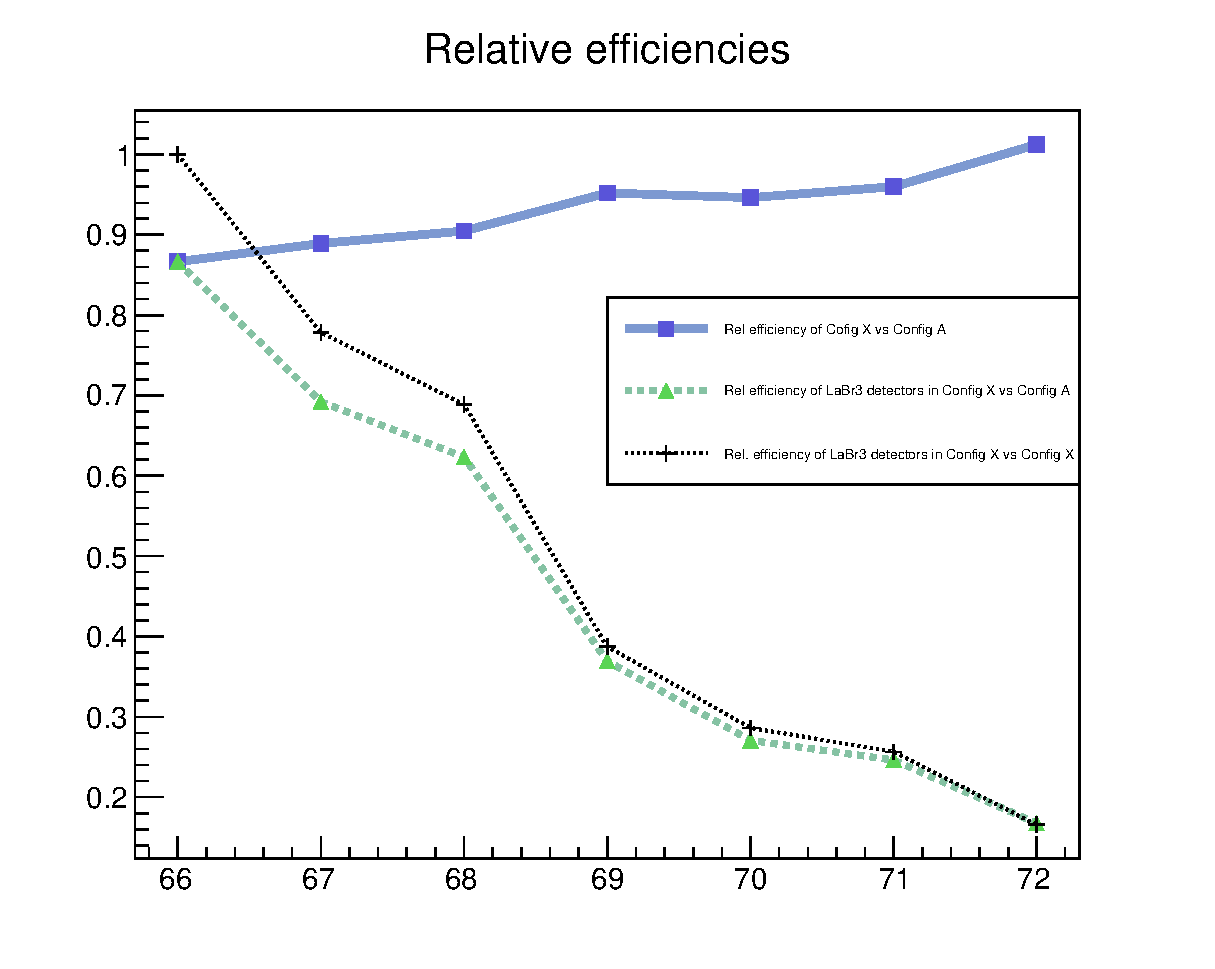
\includegraphics[width=0.7\textwidth,height=\textheight]{comp}
\end{dynamiccontents*}



\newpage
\phantom{a}

\newpage
\phantom{a}

\newpage
\phantom{a}


%%%%%% CONFIG B
\renewcommand{\Xconfig}{B}
\chapter*{Configuration \Xconfig}

\begin{dynamiccontents*}{effic}
\includegraphics[width=0.7\textwidth,height=\textheight]{Configuration\Xconfig}
\end{dynamiccontents*}

\newpage
\phantom{a}

\newpage
\phantom{a}

\newpage
\phantom{a}

\newconfig{C}

\newconfig{D}

\newconfig{E}

\newconfig{F}

\newconfig{G}

\newconfig{H}
\end{document}